\setcounter{chapter}{7}
\chapter{Limit Theorems}
\section{Introduction}
Most important theoretical results in probability theory are \textbf{limit theorems}
\section{Chebyshev's Inequality and the Weak Law of Large Numbers}
\begin{definition}[Markov's Inequality]
    If $X$ is a random variable that takes only nonnegative values, then for any value $a > 0$, \[P\{X\geq a\}\leq \frac{E[X]}{a}\]
\end{definition}
\begin{proof}For $a > 0$, let 
    \begin{equation*}
        I =
        \begin{cases}
            1 \text{ if } X\geq a   \\
            0 \text{ otherwise }
        \end{cases}
    \end{equation*} and note that since $X\geq 0$, \[I\leq\frac{x}{a}\] Taking expectations of the preceding Inequality yields \[E[I]\leq\frac{E[X]}{a}\] which proves the result since $E[i] = P\{X\geq a\}$. 
\end{proof}
\begin{definition}[Chebyshev's Inequality]
    If $X$ is a random variable with finite mean $\mu$ and variance $\sigma^2$, then for any value $k > 0$, \[P\{|X - \mu|\geq k\}\leq \frac{\sigma^2}{k^2}\]
\end{definition}
\begin{proof}
    Since $(X - \mu)^2$ is a nonnegative random variable, we can apply Markov's Inequality (with $a = k^2$) to obtain \[P\{(X - \mu)^2\geq k^2\}\leq \frac{E[(X - \mu)^2]}{k^2}\] But since $(X - \mu)^2\geq k^2$ if and only if $| X - \mu |\geq k$, the expression above is equal to \[P\{|X-\mu|\geq k\}\leq \frac{E[(X - \mu)^2]}{k^2} = \frac{\sigma^2}{k^2}\]
\end{proof}
The importance of these inequalities is that they allow us to derive bounds on probaiblity when only the mean or both the mean the variance of the probability distribution re known. If the actual distribution is known, then the desired probabiliteis could be computed exactly and no need to resort to deriving bounds from these inequlalites. 
\subsection*{Example}
Suppose that it is known that the number of items produced in a factory during a week is a random variable wtih mean $50$. \begin{enumerate}[a. ]
    \item What can be said about the probability that this week's production will exceed 75?
    \item If the variance of a week’s production is known to equal 25, then what can be said about the probability that this week’s production will be between 40 and 60?
\end{enumerate}
\subsubsection*{Solution}
Let $X$ be the number of items that will be produced in a week. 
\begin{enumerate}[a. ]
    \item By Markov's Inequality, \[P\{X > 75\}\leq\frac{E[X]}{75} = \frac{50}{75} = \frac{2}{3}\]
    \item By Chebyshev's Inequality, \[P\{|X - 50|\geq 10\}\leq\frac{\sigma^2}{10^2} = \frac{1}{4}\] Then, \[P\{|X - 50| < 10\}\geq 1 - \frac{1}{4} = \boxed{\frac{3}{4}}\] The probability that this week's prioduction will be between 40 and 60 is at least .75
\end{enumerate}
\begin{remark}
If $Var(X) = 0$, then \[P\{X = E[X]\} = 1\] In other words, the only random variables having variances equal to 0 are those that are constant with probability 1. 
\end{remark}
\begin{theorem}
    Let $X_1, X_2, \dots$ be a sequence of independent and identically distributed random variables, each having finite mean $E[X_i] = \mu$. Then, for any $\epsilon < 0$, \[P\{|\frac{X_1 + \dots + X_n}{n} - \mu|\geq \epsilon\}\rightarrow 0 as n\rightarrow \infty\]
\end{theorem}
\begin{proof}
    We shall prove the theorem only under the additional assumption that the randomv ariables have a finite variance $\sigma^2$. Now since \[E\left[\frac{X_1 + \dots + X_n}{n}\right] = \mu \text{ and Var}\left(\frac{X_1 + \dots + X_n}{n}\right) =\frac{\sigma^2}{n}\] It follows from Chebyshev's Inequality that \[P\{|\frac{X_1 + \dots + X_n}{n} - \mu|\geq\epsilon\}\leq \frac{\sigma^2}{n\epsilon^2}\] and the result is proven.
\end{proof}
\section{The Central Limit Theorem}
\begin{theorem}[The Central Limit Theorem]
    Let $X_1, X_2,\dots$ be a sequnece of independent and idnetically distriobuted random variables, each having mean $\mu$ and variance $\sigma^2$. Then the distribution of \[\frac{X_1 + \dots + X_n - n\mu}{\sigma\sqrt{n}}\] tends to the stnadard normal as $n\rightarrow\infty$. That is, for $-\infty < a < \infty$, \[P\{\frac{X_1 + \dots + X_n = n\mu}{\sigma\sqrt{n}}\leq a\}\rightarrow \frac{1}{\sqrt{2\pi}}\int^a_{-\infty} e^{-x^2/2} dx \text{ as } n\rightarrow\infty\]
\end{theorem}
The key to the CLT is the following lemma, which we state without proof. 
\begin{lemma}
Let $Z_1, Z_2, \dots$ be a sequence of randomv ariable having distribution functions $F_{Z_n}$ and moment generation functions $M_{Z_n}, n\geq 1$ and let $Z$ bea  random variable having distribution function $F_Z$ and moment generationg function $M_Z$. If $M_{Z_n}(t)\rightarrow M_Z(t)$ for all $t$, then $F_{Z_n}(t)\rightarrow F_{Z}(t)$ for alll $t$ at which $F_Z(t)$ is continuous. 
\end{lemma}
\subsection*{Example}
The number of students who enroll in a psychology course is a Poisson random variable with mean 100. The professor in charge of the course has decided that if the number enrolling is 120 or more, he will teach the course in two separate sections, whereas if fewer than 120 students enroll, he will teach all of the students together in a single section. What is the probability that the professor will have to teach two sections?
\subsubsection*{Solution}
The exact solution \[e^{-100} \sum^\infty_{i = 120} \frac{(100)^i}{i!}\] does not yield a straight numerical answer. Recall that a Poission random variable with mean 100 is the sum of 100 independent Poisson randojm variables, each wiht mean 1, we can make use of hte central limit hteorem to obtain an approximate solution. If $X$ denotes the number of students who enroll in thie cource, we have 
\begin{equation*}
    \begin{split}
        P\{X\geq 120\} &= P\{X\geq 119.5\} \text{ (the continuity correction) }\\
        &= P\{\frac{X - 100}{\sqrt{100}}\geq \frac{119.5-100}{\sqrt{100}}\}\\
        &\approx 1 - \Phi(1.95)\\
        &\approx .0256
    \end{split}
\end{equation*}
where we use the fact that the variance of a Poissonr andom variable is equal to its mean. 
\section{Strong Law of Large Numbers}
\begin{theorem}[The Strong Law of Large Numbers]
    Let $X_1, X_2, \dots $ be a sequence fo indepednent and identically distgributed randomv ariables, each having a finite mean $\mu = E[X_i]$. then, with probability 1, \[\frac{X_1 + X_2 + \cdots + X_n}{n}\rightarrow \mu \text{ as } n\rightarrow\infty\] That is the strong law of large numbers states that \[p\{\lim_{n\rightarrow\infty} (X_1 + \dots + X_n)/n = \mu\} = 1\]
\end{theorem}
An application of the strong law of large numbers, suppose that a sequence of
independent trials of some experiment is performed. Let $E$ be a fixed event of the
experiment, and denote by $P(E)$ the probability that $E$ occurs on any particular
trial. Letting
\begin{equation*}
    X_i = 
    \begin{cases}
        1 \text{ if } E \text{ occurs on the } i \text{th trial}\\
        0 \text{ if } E \text{ does not occur on the } i \text{th trial}
    \end{cases}
\end{equation*}
We have by the strong law of large numbers, that with probability 1, \[\frac{X_1 + \dots + X_n}{n}\rightarrow E[X] = P(E)\] Since  $X_1 + \dots + X_n$ represents the number of times that the event $E$ occurs in the first $n$ trials,. we interepret the previous expression as stating that with probability 1, the limiting proportion of time that the event $E$ occurs is $P(E)$.
\section{Other Inequalities and a Poisson Limit Result}
\begin{definition}[One-Sided Chebyshev Inequality]
    If $X$ is a random variable with mean $0$ and finite variance $\sigma^2$, then for any $a > 0$. \[P\{X\geq a\}\leq \frac{\sigma^2}{\sigma^2 + a^2}\]
\end{definition}
\subsection*{Example}
If the number of items produced in a factory during a week is a random variable
with mean 100 and variance 400, compute an upper bound on the probability that
this week’s production will be at least 120.
\subsubsection*{Solution}
It follows from the one-sided Chebyshev inequality that \[P\{X\geq 120\} = P\{X - 100\geq 20\}\leq \frac{400}{400 + (20)^2} = \frac{1}{2}\] The probability that this week's production will be 120 or more is at most $\frac{1}{2}$. Note that if we used Markov's inequality, then we would have got \[P\{X\geq 120\}\leq \frac{E(X)}{120} = \frac{5}{6}\] which is a much weaker bound than the one before. 
\section{The Lorenz Curve}
The Lorenz curve $L(p)$ is a plot of the fraction of the total income of a population that is earned by the $100p$ percent of the population having the lowest incomes. For instance, $L(.5)$ is the fraction of total income earned by the lower half of income earners.\\
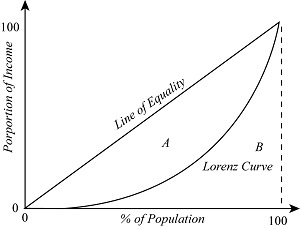
\includegraphics{LorenzCurve.jpg}[.5]